\scanpage{107}
\uline{Corollaire} 2\quad \deleted{Dans les conditions du corollaire 1} Supposons $X$ \deleted{\unsure{de plus}} quasi compact, \inserted{et $(T_0)$} et que \deleted{\unsure{toute partie}} $X$ ait une base formée d'ouverts \deleted{\unsure{quasi compacts}} rétrocompacts, qui sont q. cpts pour la topologie constructible. Soit $E$ une partie de $X$. Conditions équivalentes

a) $E$ est fermé pour la top. constructible [i.e. est intersection \deleted{finie} de parties constructibles]

b) $E$ est compact pour la top constructible, i.e. pour \unsure{$\forall$} famille de parties constructibles $(E_i)_{i\in I}$ de $X$, telle que $E\subset\bigcup_{i\in I}E_i$, il existe une sous-famille finie $J\subset I$, telle que $E\subset\bigcup_{i\in J}E_i$.

\margin{en général, \uline{partie \unsure{antifique|antifinie}} $=$ \uline{intersection de loc constructibles}. \unsure{Nature locale de la notion} ??}

\deleted{$X$ \unsure{est}} En effet, $X^{\mathrm{cons}}$ est compact, donc a) $\Longleftrightarrow$ b).

On est \unsure{convenu}\inserted{alors} que \deleted{\unsure{E}} $E$ est une \uline{partie \unsure{antifique|antifinie} de} $X$. On peut donner un énoncé analogue si $X$ n'est plus supposé q. cpt [mais satisfaisant aux deux hyp]

\diagram{\begin{tikzcd}[ampersand replacement=\&,row sep=large]
\begin{gathered}E\text{ fermé}\ \inserted{\text{dans }X^{\mathrm{cons}}}\\
[\text{i.e. intersection de parties loc. constructibles}]
\end{gathered}\arrow[d,Leftrightarrow]\\
\begin{gathered}
E\text{ loc. cpt pour la top. constructible i.e. pour }\unsure{\forall}\\
\deleted{\text{partie }\unsure{\forall}}\ U_i,\quad E\cap\unsure{U_i}\text{ satisfait la condition b}\\
\text{ci-dessus dans }U_i.
\end{gathered}
\end{tikzcd}}

\uline{Corollaire} 3\quad Dans les conditions du corollaire 2, Conditions équivalentes

a) $E$ et $X-E$ sont \unsure{antifiques|antifinies}

b) $E$ est \deleted{constructible} ouvert et fermé dans $X^{\mathrm{cons}}$

c) $E$ est constructible.

\margin{\figure{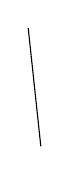
\begin{tikzpicture}\draw (0,0)--(0.16,-1.5);\end{tikzpicture}}}
\margin{106}
